\chapter{Exercise 9}
The purpose of this exercise was to understand and implement planar reflections using OpenGL.

\section{Part 1}
The setupStencil function firstly clears the stencil buffer and with
color mask set to false for all colors and alpha it sets a stencil 
for setting fields to 1 always when the stencil test passes. 
Then the function is drawing objects to that buffer. After that
color mask is again set to true for every color and stencil is set
to pass only if field is equal to 1 with read only type.
\newline
Depending on the values in drawStencil some object are drawn into 
the stencil buffer in setupStancil and some are not. After calling
this function scene will be clipped to any areas depending on which
objects were drawn.

\section{Part 2-8}
After following the instructions I managed to get a satisfactory result. 
The program is rendering both shadow and a mirror reflection (See figure \ref{fig:exercise_9_part_2_1}).
\begin{figure}[ht!]
	\begin{center}
		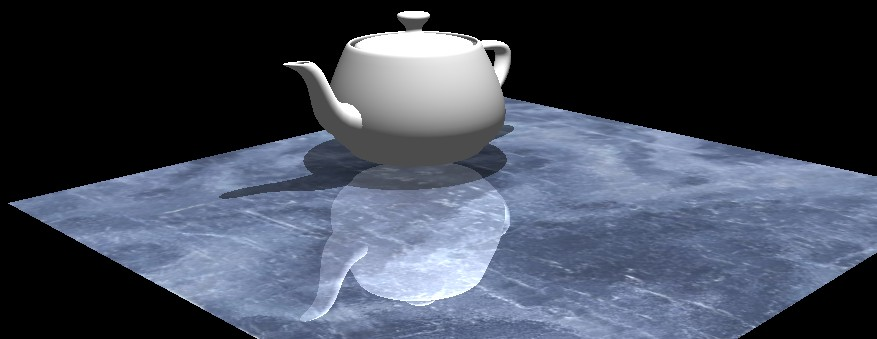
\includegraphics[width=.85\textwidth]{figures/exercise_9_part_2_1}
	\end{center}
	\vspace{-4.5ex}\caption{Exercise 9 part 2 output 1}
	\label{fig:exercise_9_part_2_1} 
\end{figure} \\
\newline
Reflected teapot rendered outside the reflecting plane is clipped away using 
a stencil buffer (See figure \ref{fig:exercise_9_part_2_2}). 
Shadow color, mirrored teapot color and a plane texture color are blended 
together as a normalized sum of colors. All of that is done by the code below.
\begin{lstlisting}[language=cpp, caption={drawPlane function}]
void drawPlane(mat4 projection, mat4 view) {
	mat4 model;
	mat4 lightViewProjection = getLightViewProjection();
	glEnable(GL_STENCIL_TEST);
    glStencilFunc(GL_ALWAYS, 1, 0xFF);
    glStencilOp(GL_KEEP, GL_KEEP, GL_REPLACE);
    glStencilMask(0xFF); 
	glColorMask(GL_FALSE, GL_FALSE, GL_FALSE, GL_FALSE);
    glDepthMask(GL_FALSE); 
    glClear(GL_STENCIL_BUFFER_BIT); 

	drawMeshObject(projection, lightViewProjection, model, view, planeObject);	

	glStencilFunc(GL_EQUAL, 1, 0xFF); 
    glStencilMask(0x00);
    glDepthMask(GL_TRUE);
	glColorMask(GL_TRUE, GL_TRUE, GL_TRUE, GL_TRUE);

	if (draw_mirror == 1) {
		drawMirror(projection, view);	
	}

	glEnable(GL_BLEND);
	glBlendFunc(GL_ONE,GL_ONE);
	drawMeshObject(projection, lightViewProjection, model, view, planeObject);
	glDisable(GL_BLEND);
	glDisable(GL_STENCIL_TEST);
}
\end{lstlisting}
\clearpage
\begin{figure}[ht!]
	\begin{center}
		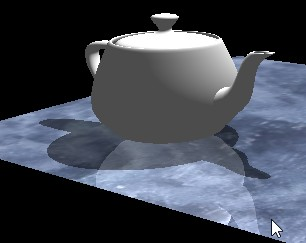
\includegraphics[width=.5\textwidth]{figures/exercise_9_part_2_2}
	\end{center}
	\vspace{-4.5ex}\caption{Exercise 9 part 2 output 2}
	\label{fig:exercise_9_part_2_2} 
\end{figure}

Using a clipPlane w coordinate I managed to clip away (discard) the unnessesary 
teapot fragments fixing the problems with shadows and reflections when a part of
the teapot is under the reflection plane. We can see the efects in the figure
\ref{fig:exercise_9_part_2_3}. In the fragment shader I used the following code
to discard unnecessary pixels: \\
\begin{lstlisting}[language=cpp, caption={clip plane - discard pixels}]
if(vWorldPos.y * clipPlane.w < clipPlane.y && clipPlane.w != 0)
{
	discard;
}
\end{lstlisting}
\begin{figure}[ht!]
	\begin{center}
		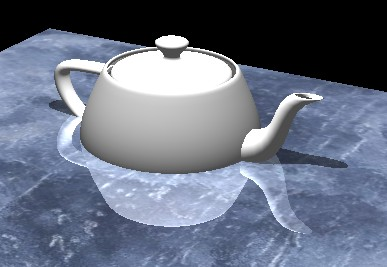
\includegraphics[width=.6\textwidth]{figures/exercise_9_part_2_3}
	\end{center}
	\vspace{-4.5ex}\caption{Exercise 9 part 2 output 3}
	\label{fig:exercise_9_part_2_3} 
\end{figure}
